\section{\rqtwo}


Our second research question aims to investigate the differences between program variants at runtime.
To answer RQ2, we execute each program/variant to collect their execution traces and execution times.
We compare each pair of programs for each programs' population by collecting \autoref{metric:stack} and \autoref{metric:time}. 

This section is organized as follows ... 

\subsection*{Program traces.}

\todo{Plot or table program traces changes }

\subsection*{Execution times.}

% Overall results
Over all diversified programs, 169 out of 239 have at least one variant with a different execution time distribution compared to the original program (P-value $<$ $0.01$ in the Mann-Withney test). This shows that we are effective at generating variants that yield significantly different execution times.

By analyzing the data, we observe the following trends.
% Lower execution times
If our tool infers control-flows as constants in the original program, then the variants execute faster than the original, sometimes by an order of magnitude. 
% Large execution times
On the other hand, as expected, if the code is augmented with more instructions, then the variants tend to run slower than the original. 

In both cases we generate a variant that has a different execution time than the original. Both cases are good from a randomization perspective, since this minimizes the certainty a malicious user can have about the program's behavior. A deeper analysis on how this phenomenon can be used to enforce security will be discussed in the answering to RQ3.

To better illustrate the differences between executions times in the variants, we dissect the execution time distributions for two programs' populations. 
% describe figures
The plots in \autoref{rq3:perf} show the execution time distributions of programs \texttt{Base64\_decode} and \texttt{Hilbert\_curve} and their variants. 
We illustrate time diversification with these 2 programs because for both, we generate unique variants with all type of transformations previously discussed in \autoref{results:rq1}.
In the plots, along the X axis, each vertical set of points represents the distribution of 100 execution times per program/variant. The Y axis represents the execution time value in milliseconds. The original program is highlighted in magenta color: the distribution of 100 execution times is given on the left-most part of the plot and its median execution time is represented as a horizontal dashed line. For each execution time distribution, the median execution time is represented as a blue dot, and the vertical gray lines represents the full distribution. The 75\% interquartile is represented by the bolder gray line. The program variants are sorted with respect to the median execution time, in descending order.



\begin{figure*}[h]
    \centering
    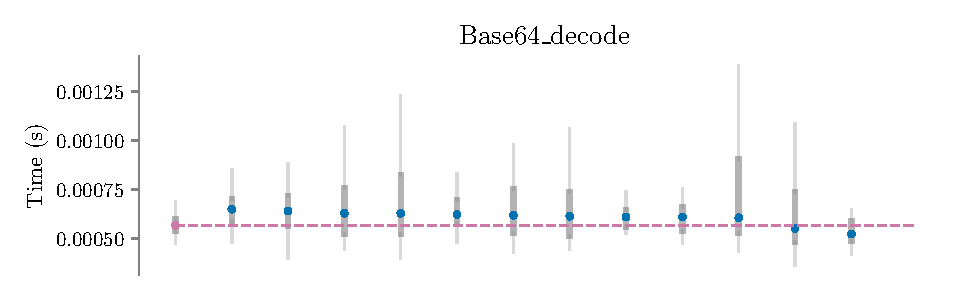
\includegraphics[width=\linewidth]{plots/base64.pdf}
    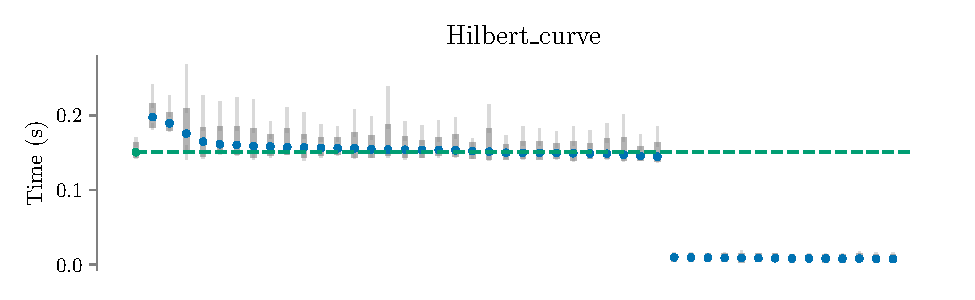
\includegraphics[width=\linewidth]{plots/hilbert_curve.pdf}
    \caption{Execution time distributions for \texttt{Base64\_decode} and \texttt{Hilbert\_curve} program and their variants in top and bottom figures respectively. Baseline execution time mean is highlighted with the magenta horiontal line. }
    \label{rq3:perf}
\end{figure*}

% explanation
For \texttt{Base64\_decode}, the majority of variants are constantly slower than the reference programs (blue dot above the magenta line). For \texttt{Hilbert\_curve}, many diversified variants are actually optimizations (blue dots below the magenta bar). The case of \texttt{Hilbert\_curve} is graphically clear, the last third represents faster variants resulting from code transformations that optimize the original program.
Our tool provides program variants in the whole spectrum of time executions, lower and faster variants compared to the original program. The developer is in charge of deciding the trade-off between taking all variants or only the ones providing the same or less execution time for sake of less overhead. 



\section{Answer to RQ2.}

% answer to RQ2
We generate variants that exhibit a significant diversity of execution times. For $169/239\,(71\%)$ of the diversified programs, at least one variant has an execution time distribution which is different compared to the execution time distribution of the original program. 


\todo{This widespread range of time execution calls for multivariant creation.}